\documentclass{oci}
\usepackage[utf8]{inputenc}
\usepackage{lipsum}
\usepackage{tikz}
\usepackage{xcolor}

\definecolor{myblue}{HTML}{bae6ff}
\def\nrows{3}
\def\ncols{5}
\newcommand{\drawnumbers}{
  \foreach \col in {1, ..., \ncols} {
    \node at (\col - 0.5, 3.35) {\col};
  }
  \foreach \row in {1, ..., \nrows} {
    \node at (-0.35, \nrows - \row + 0.5) {\row};
  }
}

\title{Figuras}

\begin{document}
\begin{problemDescription}
Cuenta la leyenda que el templo sagrado de Cumpeo alberga una cámara
secreta llena de tesoros.
%
En su última expedición, Sofía, una entrépita exploradora oriunda de
Pelotillehue, encontró un pergamino que podría contener la clave para
acceder a la cámara.
%
Lamentablemente, sus fuentes le han confirmado que Lucía, una exploradora
de Buenas Peras, también tuvo acceso al pergamino.
%
Sofía no puede soportar la idea de perder contra alguien de Buenas Peras
así que debe apresurarse para ser la primera en entrar a la cámara.

En la sala principal del templo, una de las paredes contiene un mural
formado por una grilla de $n$ filas y $m$ columnas.
%
Las filas son numeradas de arriba hacia abajo entre 1 y $n$, mientras
que las columnas de izquierda a derecha entre 1 y $m$.
%
La celda en la fila $i$ y columna $j$ es identificada con el par $(i, j)$.

Algunas de las casillas en la grilla tienen azulejos que forman
una \emph{figura conexa}.
%
Es decir, todos los azulejos son \emph{adyacentes} a al menos un azulejo.
%
Dos azulejos se consideran adyacentes si comparten un borde vertical
u horizontal.
%
La siguiente imagen muestra un ejemplo para una grilla de $3\times 5$
con azulejos en las posiciones $(3, 3)$, $(3, 4)$ y $(3, 5)$.

\begin{center}
  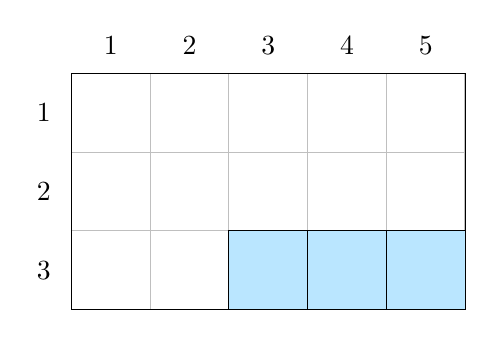
\begin{tikzpicture}
    \drawnumbers{}
    \draw[step=1, gray!50, thin] (0,0) grid (\ncols, \nrows);
    \fill[myblue, draw=black] (2, 1) rectangle (3, 0);
    \fill[myblue, draw=black] (3, 1) rectangle (4, 0);
    \fill[myblue, draw=black] (4, 1) rectangle (5, 0);
    \draw[black] (0, \nrows) rectangle (\ncols, 0);
  \end{tikzpicture}
\end{center}

En el centro de la sala, hay un tablero formado también por
una grilla de $n\times m$.
%
Sobre el tablero, hay fichas que pueden moverse entre
las casillas.
%
La cantidad de fichas es la misma que la de azulejos, pero
están dispuestas sobre el tablero en posiciones distintas.
%
La siguiente imagen muestra un ejemplo del tablero con fichas
en las posiciones $(1, 2)$, $(1, 3)$ y $(2, 3)$.


\begin{center}
  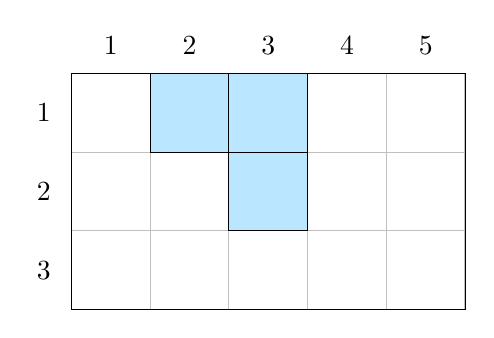
\begin{tikzpicture}
    \drawnumbers{}
    \draw[step=1, gray!50, thin] (0,0) grid (\ncols, \nrows);
    \fill[myblue, draw=black] (1, 3) rectangle (2, 2);
    \fill[myblue, draw=black] (2, 3) rectangle (3, 2);
    \fill[myblue, draw=black] (2, 2) rectangle (3, 1);
    \draw[black] (0, \nrows) rectangle (\ncols, 0);
  \end{tikzpicture}
\end{center}

De acuerdo a las instrucciones en el pergamino, para abrir
la puerta mágica a la cámara secreta hay que resolver el
acertijo del tablero.
%
El acertijo consiste en mover las fichas del tablero
hasta que coincidan con los azulejos en el mural.
%
Esto pareciera ser sencillo, pero para activar el mecanismo
mágico, las fichas deben moverse siguiendo una regla especial.
%
Específicamente, el único movimiento válido es tomar una ficha
del tablero y colocarla adyacente a otra ficha de manera que en
todo momento se forme una figura conexa.

Dado el mural y el tablero en las imágenes anteriores, la siguiente
imagen muestra una posible secuencia de movimientos que pueden usarse
para que las fichas en el tablero coincidan con los azulejos.

\begin{center}
  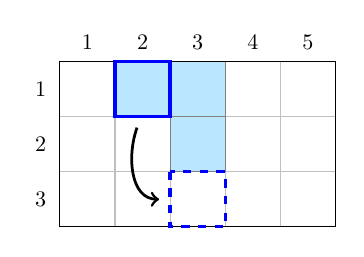
\begin{tikzpicture}[scale=0.7, every node/.style={scale=0.8}]
    \drawnumbers{}
    \draw[step=1, gray!50, thin] (0,0) grid (\ncols, \nrows);
    \fill[myblue, draw=gray] (2, 3) rectangle (3, 2);
    \fill[myblue, draw=gray] (2, 2) rectangle (3, 1);
    \draw[black] (0, \nrows) rectangle (\ncols, 0);

    \fill[myblue, draw=blue, line width=1.2pt] (1, 3) rectangle (2, 2);
    \draw[draw=blue, line width=1.2pt, dashed] (2, 1) rectangle (3, 0);
    \draw[->, black, line width=1pt] (1.4, 1.8) to[out=-110, in=180] (1.8, 0.5);
  \end{tikzpicture}
  ~
  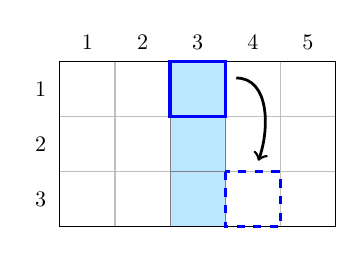
\begin{tikzpicture}[scale=0.7, every node/.style={scale=0.8}]
    \drawnumbers{}
    \draw[step=1, gray!50, thin] (0,0) grid (\ncols, \nrows);
    \fill[myblue, draw=gray] (2, 2) rectangle (3, 1);
    \fill[myblue, draw=gray] (2, 1) rectangle (3, 0);
    \draw[black] (0, \nrows) rectangle (\ncols, 0);

    \fill[myblue, draw=blue, line width=1.2pt] (2, 3) rectangle (3, 2);
    \draw[draw=blue, line width=1.2pt, dashed] (3, 1) rectangle (4, 0);
    \draw[->, black, line width=1pt] (3.2, 2.7) to[out=0, in=70] (3.6, 1.2);
  \end{tikzpicture}
  ~
  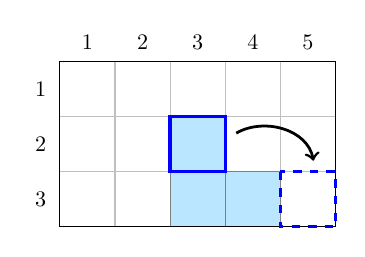
\begin{tikzpicture}[scale=0.7, every node/.style={scale=0.8}]
    \drawnumbers{}
    \draw[step=1, gray!50, thin] (0,0) grid (\ncols, \nrows);
    \fill[myblue, draw=gray] (2, 1) rectangle (3, 0);
    \fill[myblue, draw=gray] (3, 1) rectangle (4, 0);
    \draw[black] (0, \nrows) rectangle (\ncols, 0);

    \fill[myblue, draw=blue, line width=1.2pt] (2, 2) rectangle (3, 1);
    \draw[draw=blue, line width=1.2pt, dashed] (4, 1) rectangle (5, 0);
    \draw[->, black, line width=1pt] (3.2, 1.7) to[out=30, in=100] (4.6, 1.2);
  \end{tikzpicture}
  ~
  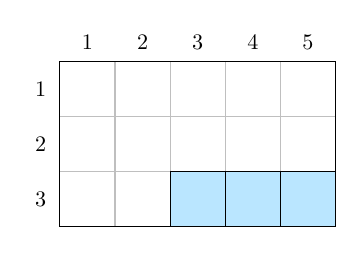
\begin{tikzpicture}[scale=0.7, every node/.style={scale=0.8}]
    \drawnumbers{}
    \draw[step=1, gray!50, thin] (0,0) grid (\ncols, \nrows);
    \fill[myblue, draw=black] (2, 1) rectangle (3, 0);
    \fill[myblue, draw=black] (3, 1) rectangle (4, 0);
    \fill[myblue, draw=black] (4, 1) rectangle (5, 0);
    \draw[black] (0, \nrows) rectangle (\ncols, 0);
  \end{tikzpicture}
\end{center}
En el primer movimiento la ficha en la posición $(1, 2)$ se mueve a la
posición $(3, 3)$.
%
Posteriormente, la ficha en la posición $(1, 3)$ se mueve a la posición
$(3, 4)$.
%
Finalmente, la ficha en la posición $(2, 3)$ se mueve a la posición  $(3, 5)$.

Sofía quiere resolver el acertijo lo más rápido posible, pero está
teniendo problemas.
En particular, le gustaría saber la mínima cantidad de movimientos
en que es posible hacer coincidir las fichas con los azulejos.
?`Podrías ayudarla?

\end{problemDescription}

\begin{inputDescription}
  La primera línea de la entrada contiene dos enteros $n$ y $m$ ($n \times m \leq 2 \times 10^5$)
  correspondientes a las dimensiones del tablero y el mural.
  Luego vienen $2 \times n$ líneas describiendo el tablero y el mural.

  Las primeras $n$ líneas describen el tablero.
  %
  Cada línea contiene $m$ enteros iguales a 0 o 1.
  %
  El $j$-ésimo entero en la línea $i$ describe la casilla $(i, j)$ del tablero.
  %
  Un 1 indica que la posición contiene una ficha y un 0 indica que la casilla
  está vacía.

  Las últimas $n$ líneas describen el mural usando el mismo formato para describir
  las casillas que tienen azulejos.

  Se garantiza que la cantidad de unos en el tablero y en el mural será la misma.
\end{inputDescription}

\begin{outputDescription}
La salida debe contener un entero, el número mínimo de movimientos
requeridos para mover las casillas de forma que coincidan con
los azulejos.
% En caso de que no se pueda, imprimir "IMPOSIBLE" (sin las comillas).
\end{outputDescription}

\begin{scoreDescription}
  \subtask{15} Se probarán varios casos donde $n=1$ y $m\leq 2\times 10^3$.
  \subtask{25} Se probarán varios casos donde $n\times m \leq 2\times 10^3$.
  \subtask{60} Se probarán varios casos sin restricciones adicionales.
\end{scoreDescription}

\begin{sampleDescription}
\sampleIO{sample-1}
% \sampleIO{sample-2}
\end{sampleDescription}

\end{document}
